\documentclass[a4paper, 12pt]{article}%тип документа

%отступы
\usepackage[left=2cm,right=2cm,top=2cm,bottom=3cm,bindingoffset=0cm]{geometry}

%Русский язык
\usepackage[T2A]{fontenc} %кодировка
\usepackage[utf8]{inputenc} %кодировка исходного кода
\usepackage[english,russian]{babel} %локализация и переносы

%Вставка картинок
\usepackage{wrapfig}
\usepackage{graphicx}
\graphicspath{{images/}}
\DeclareGraphicsExtensions{.pdf,.png,.jpg}

%оглавление
\usepackage{titlesec}
\titlespacing{\chapter}{0pt}{-30pt}{12pt}
\titlespacing{\section}{\parindent}{5mm}{5mm}
\titlespacing{\subsection}{\parindent}{5mm}{5mm}
\usepackage{setspace}

%Графики
\usepackage{multirow}
\usepackage{pgfplots}
\pgfplotsset{compat=1.9}

%Математика
\usepackage{amsmath, amsfonts, amssymb, amsthm, mathtools}

%Стиль страницы
\usepackage{fancyhdr}
\pagestyle{fancy}

\begin{document}

\begin{titlepage}

\begin{center}
%\vspace*{1cm}
\large\textbf{Московский Физико-Технический Институт}\\
\large\textbf{(государственный университет)}
\vfill
\line(1,0){430}\\[1mm]
\huge\textbf{Работа 5.8.1}\\
\line(1,0){430}\\[1mm]
\vfill
\large Сибгатуллин Булат, ФРКТ\\
\end{center}

\end{titlepage}
\fancyhead[L] {Работа 5.8.1}
\noindent \textbf{Цель работы:} \\
\indent При помощи модели абсолютно чёрного тела проведение измерения температуры оптическим пирометром с исчезающей нитью и термопарой. Исследование излучение накалённых тел с различной испускательной способностью. Определение постоянных Планка и Стефана-Больцмана.
\noindent \textbf{В работе используются:} \\
\indent Оптический пирометр, модель абсолютно чёрного тела, образцы колец, вольфрамовая лампа, неоновая лампа, блок питания, цифровые вольтметры.

\section{Описание работы}
Для измерения температуры разогретых тел, удалённых от наблюдателя, применяют методы оптической пирометрии, основанные на использовании зависимости испускательной способности исследуемого тела от температуры. Различают три температуры, функционально связанные с истинной термодинамической температурой и излучательной способностью тела: радиационную $T_{rad}$, цветовую $T_{col}$ и яркостную $T_{br}$.

В работе измеряется яркостная температура. \textbf{Яркостная температура} - это температура абсолютно чёрного тела, при которой его спектральная испускательная способность равна спектральной испускательной способности исследуемого тела при той же длине волны.
 Измерение яркостной температуры раскалённого тела производится при помощи оптического пирометра с исчезающей нитью, основанного на визуальном сравнении яркости раскалённой нити с яркостью изображения исследуемого тела.
 
Яркостная температура тела всегда ниже его термодинамической температуры. Это связано с тем, что любое нечёрное тело излучает меньше, чем АЧТ при той же температуре. Зависимость между яркостной и термодинамической температурами вольфрама приведена на рис. 1

\begin{figure}[h]
    \centering
    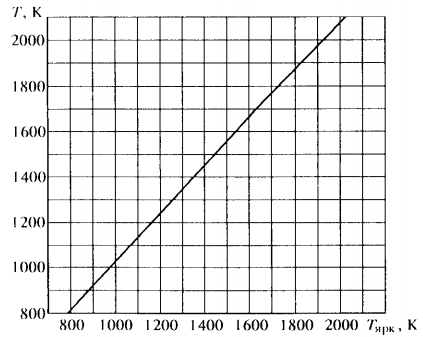
\includegraphics[width=10cm]{fig2.PNG}
    \caption{График зависимости $T = f(T_br)$ для вольфрам}
    \label{fig:vac}
\end{figure}

По результатам измерений мощности излучения вольфрамовой нити можно судить о справедливости закона Стефана-Больцмана. Если бы нить излучала как АЧТ, то баланс потребляемой и излучаемой энергии определялся бы соотношением 
\begin{equation}
    W = \sigma S (T^4 - T_0^4),
\end{equation}
где $W$ - потребляемая нитью электрическая мощность, $S$ - площадь излучающей поверхности нити, $T$ - температура нити, $T_0$ - температура окружающей среды. Однако вольфрамовая нить излучает как серое тел, и излучение её ослаблено по сравнению с АЧТ в $\varepsilon_T$ раз для любой волны при данной температуре тела Т. Тогда предположив, что нить излучает как серое тело и с учётом того, что $T_0 \ll T$, выражение (1) можно переписать в виде
\begin{equation}
    W = \varepsilon_T S \sigma T^4
\end{equation}
В справедливости закона Стефана-Больцмана можно убедиться, построив график зависимости $W(T)$ в логарифмическом масштабе и по углу наклона определить показатель степени $n$ исследуемой температурной зависимости. В пределах погрешности показатель степени должен быть близок к четырём. \par
Также из формулы (2) можно определить постоянную Стефана-Больцмана.

\section{Экспериментальная установка}

\begin{figure}[h]
    \centering
    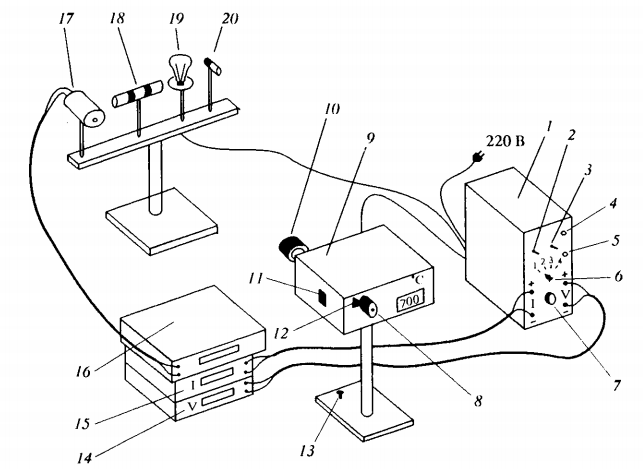
\includegraphics[width=11cm]{fig1.PNG}
    \caption{Схема экспериментальной установки: 1 - блок питания; 2 - тумблер включения питания образцов; 3 - тумблер нагрева нити пирометра; 4 - кнопка "Нагрев нити"; 5 - кнопка "охлаждение нити"; 6 - тумблер переключения образцов; 7 - регулятор мощности нагрева образцов; 8 - окуляр пирометра; 9 - корпус пирометра; 10 - объектив пирометра; 11 - переключение диапазонов; 12 - ручка смещения красного светофильтра; 13 - регулировочный винт; 14 - вольтметр (напряжение на лампе накаливания); 15 - амперметр (ток через образцы); 16 - вольтметр в цепи термопары; 17 - модель АЧТ; 18 трубка с кольцами из материалов с различной излучательной способностью; 19 - лампа накаливания; 20 - неоновая лампочка}
    \label{fig:vac}
\end{figure}

Исследуемые в работе образцы:
\begin{itemize}
    \item \textbf{модель абсолютно чёрного тела} - керамическая трубка, закрытая с одного конца и окружённая для теплоизоляции внешним кожухом. Температура в трубке измеряется с помощью термопары хромель-алюмель
    \item \textbf{керамическая трубка с набором колец из различных материалов}, нагреваемая изнутри нихромовой спиралью. Материалы колец имеют различную излучательную способность
    \item \textbf{вольфрамовая нить электрической лампочки}
\end{itemize}

\section{Ход работы}
\begin{enumerate}

\subsection{Изучение работы оптического пирометра}
\item Выведем оба светофильтра пирометра. Пожключим питание образцов и пирометра к сети 220В. 

\item Нажмем кнопку 4 и удерживая ее увеличим температуру пирометра до 900-950$^{\circ}C$. Перемещением окуляра добьемся увеличения резкости нити в поле зрения.

\item Введем красный светофильтр пирометра. Нажмем кнопку 4 или 5 и повышая или понижая ток добьемся исчезновения изображения нити на фоне изображения раскаленной модели дна АЧТ.

\item Определим по шкале пирометра значение яркостной температуры модели АЧТ. Получим $T_{\text{пирометра}} = 984^{\circ} C \: T_{\text{термопары}} = 932^{\circ} C$

Получаем погрешность измерения приблизительно равную $4,3 \%$. Это означает, что пирометр работает исправно.


\subsection{Измерение яркостной температуры раскаленных тел}
\item Направим пирометр на поверхность керамической трубки с кольцами из различных материалов. Измерим яркостную температуру поверхности трубки и каждого из колец. Результаты запишем в таблицу:

\begin{center}
\begin{tabular}{|c|c|}
\hline 
$T_{\text{тр}}, ^{\circ} C$ & 870 \\ 
\hline 
$T_{\text{к1}}, ^{\circ} C$ & 820 \\ 
\hline 
$T_{\text{к2}}, ^{\circ} C$ & 750 \\ 
\hline 
\end{tabular} 
\end{center}

Видим, что хоть трубка и два кольца накалены до одинаковой термодинамической температуры, их яркостные температуры различаются. Это происходит из-за того, что яркостная и термодинамическая температура связаны через спектральный коэффициент поглощения, который у разных материалов различный.

\subsection{Проверка закона Стефана-Больцмана}
\item Направить пирометр на нить лампы накаливания.

\item Увеличивая при помощи руки 7 накал нити лампы измерять пирометром яркостную температуру нити каждые 100$^{\circ}C$. При каждом измерении температуры также записываем величину тока и падение напрядения через лампу. Результаты запишем в таблицу

\begin{figure}[h]
    \centering
    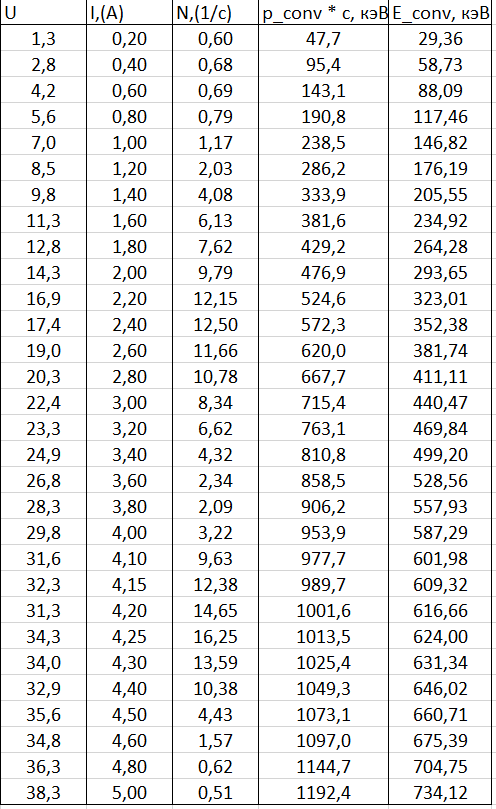
\includegraphics[width=10cm]{table_1.PNG}
    \caption{Проверка закона Стефана-Больцмана}
    \label{fig:table_1}
\end{figure}

Теперь построим график ln(W)от ln(T), причем мощность запишем как $W = U \cdot I$

\begin{figure}[h]
    \centering
    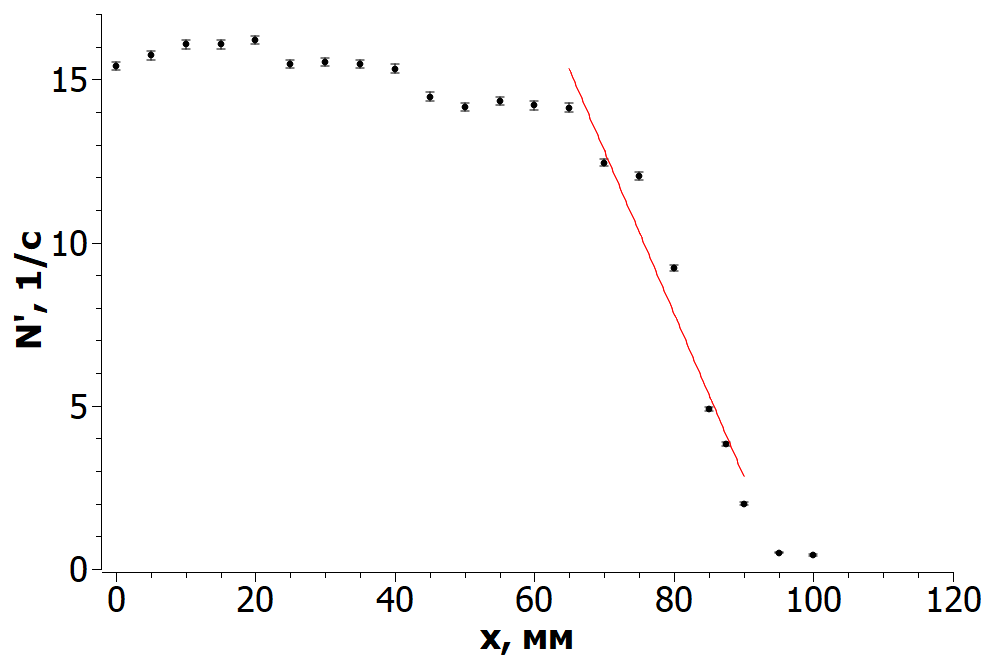
\includegraphics[width=10cm]{graph_1.PNG}
    \caption{Зависимость ln(W) от ln(T)}
    \label{fig:table_1}
\end{figure}

Получили зависимость вида $y = ax + b$:

\[a = 3,97 \pm 0,15\]

\[b = -30,9 \pm 1,2\]

Также зависимость $W = f(T)$ в логарифмическом масштабе можно представить как $ln(W) = ln(\varepsilon_T \sigma S) + n\cdot ln(T)$. Следовательно коэффициент наклона будет отражать степень n. У нас она получилась равной 3,97 при теоретическом значении 4. То есть значения совпали в пределах погрешности (если учитывать $4 \%$ погрешность пирометра).

Теперь из значения b оценим постоянную Стефана-Больцмана ($\sigma$):

\[b = ln(\varepsilon_T \sigma S) \: \Rightarrow \: \sigma = \frac{e^b}{\varepsilon_T S}\]

Здесь $S = 0,36 cm^2$, а $\varepsilon_T = 0,439$ для 1800 К, 0,437 для 1900 К и 0,435 для 2000 К. Тогда для данных значений температур мы получим следующие постоянные Стефана-Больцмана:

\begin{center}
\begin{tabular}{|c|c|c|}
\hline 
$T, K$ & $\sigma, \frac{\text{Вт}}{\text{м}^2 \cdot \text{К}^4}$ & $\sigma_{\sigma}, \frac{\text{Вт}}{\text{м}^2 \cdot \text{К}^4}$ \\ 
\hline 
1800 & $4,32\cdot 10^{-13}$ & $0,22\cdot 10^{-13}$ \\ 
\hline 
1900 & $4,08\cdot 10^{-13}$ & $0,21\cdot 10^{-13}$ \\ 
\hline 
2000 & $3,87\cdot 10^{-13}$ & $0,20\cdot 10^{-13}$ \\ 
\hline 
\end{tabular} 
\end{center}

Для сравнения теоретической значение для данной величины равно: 

\[\sigma_th = 5,67 \cdot 10^{-12} \frac{\text{Вт}}{\text{м}^2 \cdot \text{К}^4}\]

Потом найдем постоянную планку для температуры в 1900К по формуле:

\[h = \sqrt[3]{\frac{2\pi^5 k_{\text{б}}^4}{15 c^2 \sigma}}\]

\[h = 3,42 \cdot 10^{-32} \pm 0,18\cdot 10^{-32} \: \text{Дж} \cdot \text{с}\]

\subsection{Измерение яркостной температуры неоновой лампочки}

\item Термодинамическая температура неоновой лампочки примерно равна комнатной и не соответствует ее яркостной температуре ($881^{\circ} C$). Суть в том, что неоновая лампочка впринципе не является моделью черного тела, а ее излучение носит совершенно другую природу. То, что ее свет имеет такой же цвет, что и нагретое АЧТ - совпадение.

\end{enumerate}

\section{Вывод}

Видим, что наши полученные данные для постоянной Стефана-Больцмана $\sigma$ и постоянной планки $h$ вообще не сходятся с теоретическими значениями. Это может происходить из-за того, что пирометр все же был плохо настроен. Также я мог плохо определять совпадение двух цветов (при определении яркостной температуры), что тоже может сказаться на определении результатов.

При измерении яркостной температуры раскаленных тел и яркостной температуры неоновой лампочки подтвердили теоретические сведения.

\end{document}